\begin{abstract}
% =============================================================================
%X What are we doing
Deliberating takes time. In real-time settings, that time is not free.
Standard reinforcement learning (RL) sidesteps this as the environment waits indefinitely
for the agent's decision.
Instead, here, we study environments that progress while waiting for the agent's action, which naturally creates a \textit{cost of deliberation}.
%Y why is this hard
Crucially, there are state-dependent trade-offs between deliberating longer and reacting quickly. Furthermore, deliberating how much to deliberate, in the limit, risks complete paralysis.
% Z our genius insight
We resolve this with a two-step process.
First, we train a standard MCTS policy.
Second, we train a \textit{lightweight} gating policy that decides how many search steps to invest at each state. Our gating policy consistently outperforms fixed-budget baselines and hand-coded heuristics while using less average compute.
We validate the full pipeline in a true two-GPU real-time setup across real-time Pac-Man, Tetris, Snake, Speed Hex, and Speed Go.

\end{abstract}

\section{Introduction}
% =============================================================================

Real-world decision-makers operate under time pressure.
In speed chess, the world does not pause while a player thinks: the clock
runs, the opponent's plan develops, and a strong move played too late may be
worse than a weaker move played on time.
Standard reinforcement learning (RL) sidesteps this entirely.
The Markov Decision Process (MDP) framework assumes the environment waits for
the agent, so deliberation is free and an agent may take arbitrarily long to
choose an action.

This assumption breaks down in real-time settings, where the world keeps
progressing while the agent decides.
The cost of deliberation in such settings is not abstract compute usage or
latency in isolation, but \emph{environmental progression}: ghosts close in,
pieces fall, clocks deplete.
A perfect action that arrives one frame too late may be worse than a timely,
good-enough action.

This creates a spectrum of regimes.
At one extreme, the agent reacts immediately to every frame.
At the other, it thinks deeply and falls behind while the environment
continues to evolve.
We study the intermediate regime in which the agent dynamically chooses how
long to think before acting.
We refer to this setting as \emph{variable-delay real-time RL}.

We instantiate this regime with planning-based agents.
Specifically, we use AlphaZero-style models~\citep{silver2018general} that run
Monte Carlo Tree Search (MCTS) at decision time to improve action selection
(see Appendix~\ref{app:az_primer} for a complete description).
The number of MCTS simulations is a natural planning-budget knob: more
simulations can improve the action estimate, but they also take longer to run.
We verify empirically that planning quality and inference latency co-scale over
the simulation ranges we study (Figure~\ref{fig:scaling}).
This makes simulation count the central resource-allocation decision in the
real-time setting.

The key problem is therefore \emph{metareasoning}: deciding not only what
action to take, but how much computation that decision deserves.
We address this with a lightweight \emph{gating policy}, trained with PPO on
top of a \emph{frozen} AlphaZero planner, that maps each state to a budget
$K \in \Kset$.
While the planner runs, the agent executes fast filler actions: reflex actions
in committed-action environments and no-ops in clock environments.
The gate's forward pass is orders of magnitude cheaper than MCTS, so the
meta-decision itself adds negligible real-time cost.

We study this setting across two environment classes.
In \emph{committed-action environments} (Pac-Man, real-time Tetris, Snake), the
world evolves while planning is in progress.
In \emph{clock environments} (Speed Hex, Speed Go), the board is static while
thinking, but each player has an explicit clock that depletes with deliberation.
Both settings make the cost of thinking real by construction, though through
different physical mechanisms.

Our contributions are:
\begin{enumerate}
  \item \textbf{Variable-delay real-time RL.}
    We study a setting in which the agent chooses how long to deliberate at
    each decision point, and instantiate it through two environment classes:
    committed-action progression and explicit clocks.
  \item \textbf{Adaptive gating for MCTS budgets.}
    We train a lightweight gating policy on top of a frozen AlphaZero planner
    that selects a state-dependent planning budget $K \in \Kset$.
  \item \textbf{Empirical and deployment validation.}
    Across five environments, the gating policy outperforms fixed-budget and
    heuristic baselines, and the learned policy transfers directly to true
    two-GPU asynchronous deployment with no architectural change.
\end{enumerate}

The learned strategies are interpretable and state-dependent: the gate plans
more deeply in high-stakes situations and reacts quickly elsewhere.
In a true two-GPU deployment, the same trained policy transfers cleanly, and
gate inference adds negligible overhead relative to MCTS latency.

\begin{figure}[t]
  \centering
  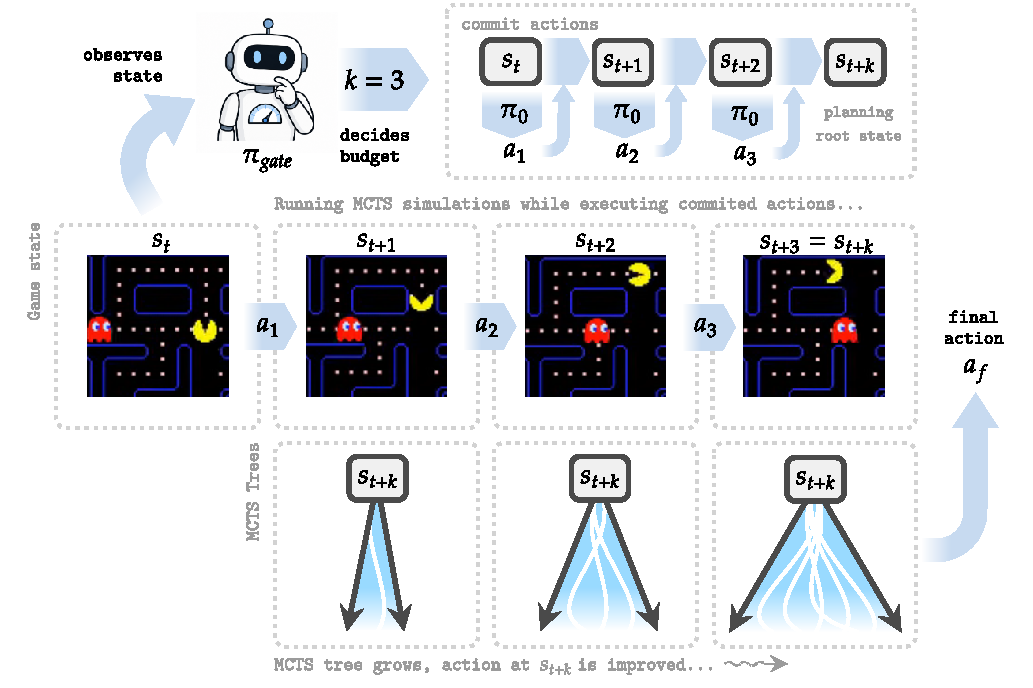
\includegraphics[width=\linewidth]{figures/realtime-rl-gating-diagram.pdf}
  \caption{
    The gating policy chooses whether to react immediately or spend time
    planning.
    Given the current state, a planning budget $K$ is selected, which
    determines how long MCTS runs and, in committed-action environments,
    how many reflex actions are taken.
  }
  \label{fig:realtime-rl-gating-diagram}
\end{figure}
